\chapter{System Architecture}

\section{System Architecture Overview}
\label{system_architecture_overview}
The system is designed as a modular client-server architecture for detecting and redacting sensitive content in both still images and video. At a high level, the architecture consists of a frontend, a backend/API layer, and separate processing components for detection and redaction.

\begin{figure}[H]
    \centering
    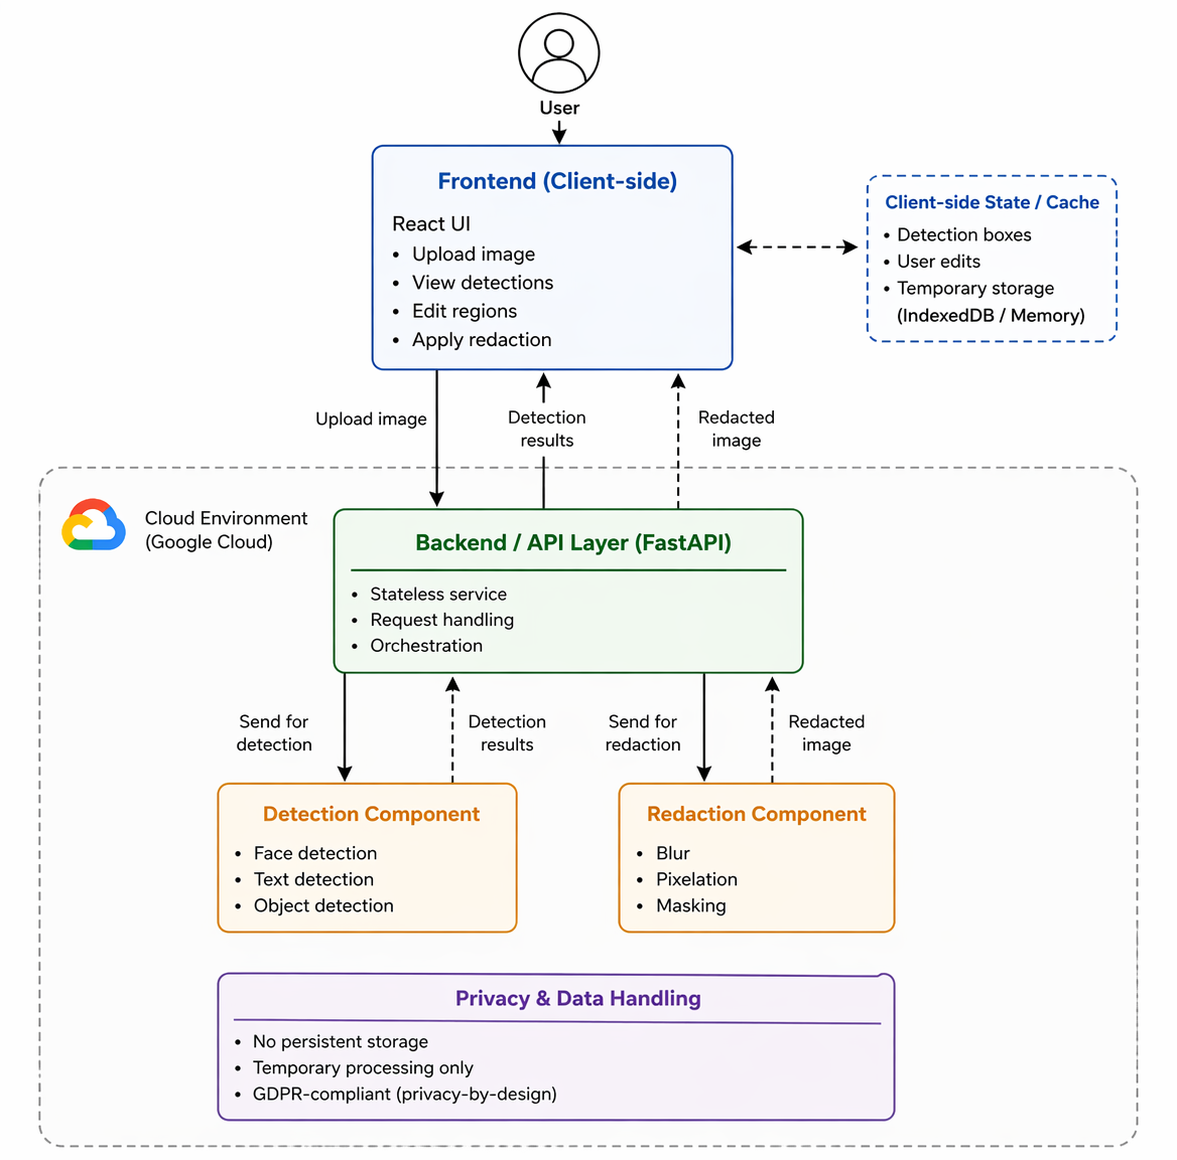
\includegraphics[width=0.85\textwidth]{figures/images/chapter-5/SystemArchitectureOverview.png}
    \caption{High-level system architecture of the proposed solution. Created by the authors, with AI-assisted refinement.}
    \label{fig:system_architecture_overview}
\end{figure}

Figure~\ref{fig:system_architecture_overview} provides an overview of the main architectural elements and their relationships. The following subsections describe the design principles and system components in more detail.

\methodheading{Architectural Design}
\label{architecture_design}
The system follows a layered architectural design, where each layer has a specific responsibility and communicates with adjacent layers. This design reduces system complexity and enables independent development of components \cite{shaw1996software}. It also simplifies debugging and testing, as each layer can be evaluated in isolation.

\begin{itemize}
    \item \textbf{Presentation Layer (Frontend):} Handles user interaction and displays results.
    \item \textbf{Application Layer (Backend):} Manages requests and coordinates processing.
    \item \textbf{Processing Layer:} Performs detection and redaction operations.
\end{itemize}

\methodheading{Design Principles}
\label{design_principles}
The architecture is guided by several design principles to ensure robustness and long-term maintainability.

A client-server architecture is used to separate user interaction from processing
logic. The client is responsible for the user interface, while the server handles
data processing and computational tasks \cite{clientserverUW}. This separation allows
computationally intensive operations, such as machine learning inference, to be
performed on the server side.

Separation of concerns is applied by assigning distinct responsibilities to each component. In particular, detection and redaction are implemented as separate modules, allowing improvements to one part of the pipeline without affecting the other. This reduces coupling and simplifies future extensions \cite{martin2017}.

Modularity is emphasized to support extensibility. For example, the detection module can be replaced or upgraded as new machine learning models become available, without requiring changes to the frontend or backend interfaces. This follows principles of modular design and loose coupling, improving maintainability and flexibility \cite{martin2017}.

The backend is designed to be stateless, meaning that each request is processed
independently. As a result, deployment is simplified and the system can scale
horizontally by distributing requests across multiple instances \cite{aws_stateless}.

Privacy is a key design consideration. By avoiding persistent storage of sensitive
data, the system minimizes the risk of data exposure and aligns with data
minimization principles defined in the GDPR \cite{gdpr}. This introduces a trade-off, as features such as history tracking or persistent sessions are limited, but this was considered
acceptable given the sensitivity of the processed data.

Overall, the chosen architecture reflects a balance between performance, usability, and privacy, where real-time interaction and user control are prioritized over fully automated processing.

\section{System Components}

Section~\ref{system_architecture_overview} presented the system from a layered architectural perspective. This section complements that view by describing the system in terms of functional components and their responsibilities.

The system consists of four primary components: the User Interface (UI), the Detection component, the Redaction component, and the API layer. These components are designed according to the principles discussed in
Subsection~\ref{design_principles}.

\methodheading{User Interface (UI)}

The User Interface (UI) is a web-based frontend responsible for presenting
detection results and enabling user interaction with the system. It serves as the
primary point of interaction between the user and the processing pipeline.

A central aspect of the UI is the workspace, which provides an interactive view
of uploaded images and detected regions. Users can inspect and validate detection
results before redaction is applied, supporting a human-in-the-loop workflow.
This is further discussed in Chapter~\ref{user_interface_and_usability}.

The UI communicates with the backend through the API layer and presents processed results to the user. It is responsible for maintaining a consistent interaction state as detection results are reviewed or redaction is applied.

The UI supports the privacy-oriented design described in
Subsection~\ref{design_principles} by handling sensitive user data primarily on the client side.

\methodheading{Detection and Redaction Component}

A central backend processing component in the system is organized around two
main workflows: detection and redaction. As illustrated in
Figure~\ref{fig:api_workflows}, these workflows follow the same overall
structure for both still images and video. In both cases, the media is processed
through the same core stages for analysis, sensitive-region identification, and
redaction. The main difference is that video processing operates across multiple
frames, and the frame-level results must be accumulated before being returned to
the frontend.

Figure~\ref{fig:api_workflows}(a) shows the high-level detection workflow. After
input media is received by the API, it is decoded and may optionally undergo
preprocessing. The media is then passed to multiple detection components, which
can operate in parallel. Their outputs are subsequently normalized into a
consistent format before being returned through the API layer. For still images,
this produces a direct detection result. For video, the same workflow is applied
to relevant frames, and the frame-level detections are collected into a unified
response.

\begin{figure}[H]
\centering

\begin{subfigure}[t]{0.48\textwidth}
    \centering
    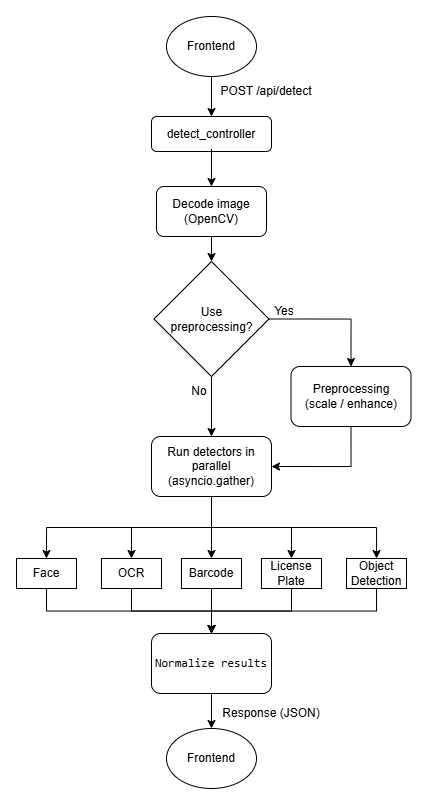
\includegraphics[width=\textwidth]{figures/images/chapter-5/detection-api-flow-v2.png}
    \caption{Detection pipeline showing image processing, optional preprocessing, parallel execution of detection models, and result normalization.}
    \label{fig:detection_api_flow_v2}
\end{subfigure}
\hfill
\begin{subfigure}[t]{0.48\textwidth}
    \centering
    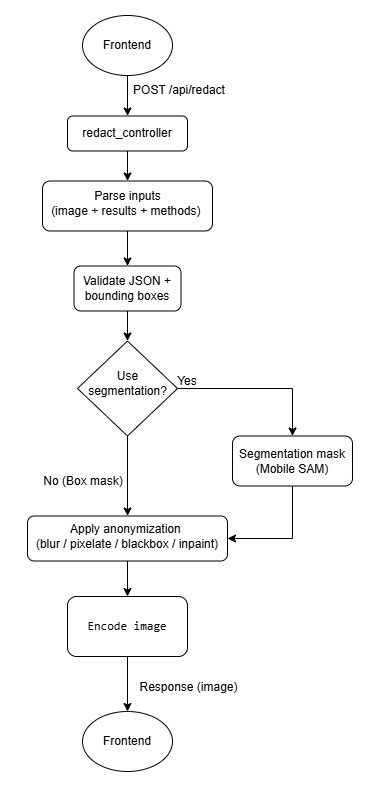
\includegraphics[width=\textwidth]{figures/images/chapter-5/redaction-api-flow-v2.png}
    \caption{Redaction pipeline showing input validation, optional segmentation, and application of anonymization techniques.}
    \label{fig:redaction_api_flow_v2}
\end{subfigure}

\caption{Overview of detection and redaction workflows in the backend system.}
\label{fig:api_workflows}
\end{figure}

Rather than applying redaction automatically, the detection results are sent to
the UI for user review and adjustment. This improves reliability in cases where
automated detection may be incomplete or imprecise.

Figure~\ref{fig:api_workflows}(b) shows the corresponding redaction workflow.
In this stage, the backend receives both the input media and the validated
detection results, applies input validation, and executes the selected
anonymization method. Depending on the selected strategy, redaction may be
based on bounding boxes or segmentation masks. For still images, redaction is
applied directly to the image. For video, the same workflow is applied frame by
frame, after which the processed frames are recombined into the final redacted
video.

This design makes it possible to separate detection from redaction as two
independent but connected stages. Such a separation improves modularity and
also allows detection results to be reused for visualization, inspection, or
later anonymization.

\methodheading{API Layer}

The API layer defines the communication interface between the frontend and the
backend processing components. It exposes detection and redaction functionality
through well-defined endpoints, allowing the UI to interact with the processing
pipeline without depending on its internal implementation. The API follows the
stateless and privacy-oriented design principles described in
Subsection~\ref{design_principles}.

The API is organized using a modular structure in which different tasks are
handled by dedicated controllers. In particular, detection and redaction are
exposed through separate routes, which improves maintainability and helps
distinguish between different processing tasks, including image-based and
video-based workflows.

\begin{figure}[H]
\centering
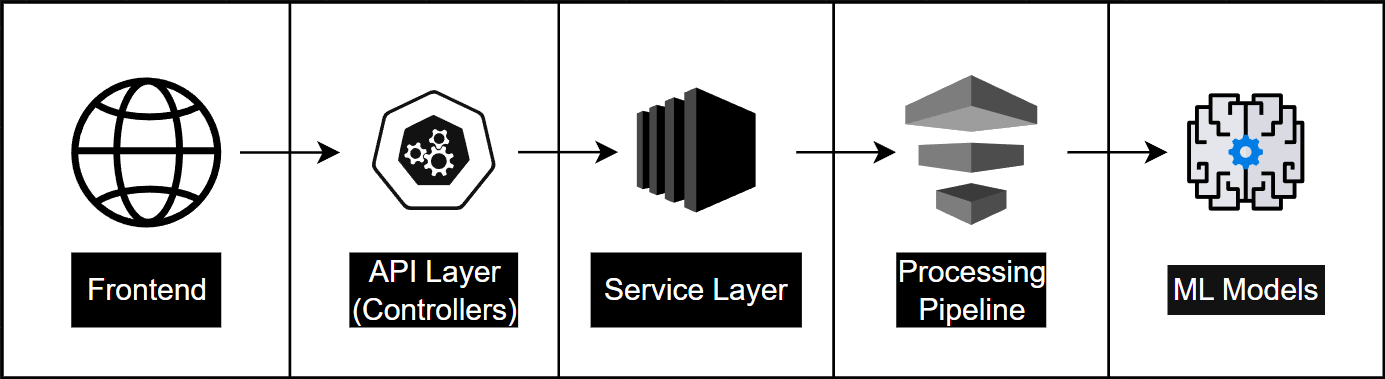
\includegraphics[width=14cm]{figures/images/chapter-5/backend_architecture_diagram.png}
\caption{Overview of the backend architecture showing the API layer, service layer, processing pipeline, and machine learning components.}
\label{fig:backend_architecture_diagram}
\end{figure}

The frontend communicates with the API layer, which forwards
requests to the service layer and the underlying processing pipeline (Figure~\ref{fig:backend_architecture_diagram}).
This reflects a layered design in which request handling, application logic, and
machine learning inference are separated into distinct responsibilities.


\methodheading{Machine Learning Development Process}

In addition to the deployed application components, the project also included a
separate development process for custom machine learning models. This process was required for the barcode and license plate detectors, as well
as the custom NER model used for text classification in the system, and formed an important part of the overall solution architecture.

As illustrated in Figure~\ref{fig:ml_pipeline}, the process consists of dataset
preparation, model training, evaluation, and deployment. In practice, this
meant that datasets had to be collected and standardized, models had to be
trained and evaluated in a dedicated development environment, and selected model
artifacts were then integrated into the SafeVision backend for inference.

\begin{figure}[H]
\centering
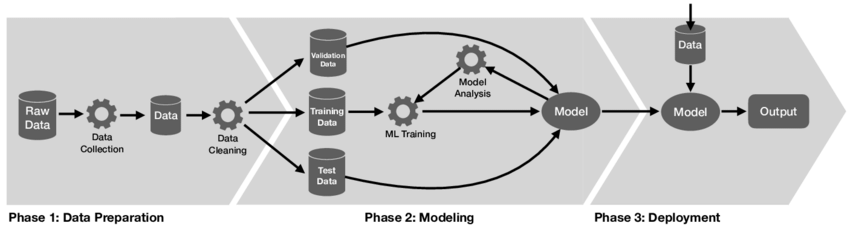
\includegraphics[width=0.9\textwidth]{figures/images/chapter-5/machine-learning-pipeline.png}
\caption{General machine learning pipeline consisting of data preparation, model training, evaluation, and deployment phases (adapted from \cite{ml_pipeline_source}).}
\label{fig:ml_pipeline}
\end{figure}

This development process was kept separate from the deployed application in
order to reduce coupling between experimental model development and the
production-oriented system. While the SafeVision application is responsible for
inference, redaction, and user interaction, the machine learning development
process focuses on preparing data, training models, and validating model
performance before integration into the deployed backend.

The technical tools, environments, and repository structure used to support this
process are described in Chapter~\ref{chap:technologies_and_methodologies}, while the
concrete implementation of dataset preparation, training, and model integration
is presented in Chapter~\ref{chap:implementation_details}.


\section{Deployment Architecture}

The deployment architecture describes how SafeVision is made available as a
web-based system and how its main components are organized in operation. In
line with the overall client--server architecture, the system is deployed as two
separate parts: a browser-based frontend client and a backend service
responsible for API handling and processing tasks. The backend handles
detection, redaction, and related processing tasks for both still images and
video. This includes model inference, redaction processing, and media-specific
workflow handling.

\begin{figure}[H]
\centering
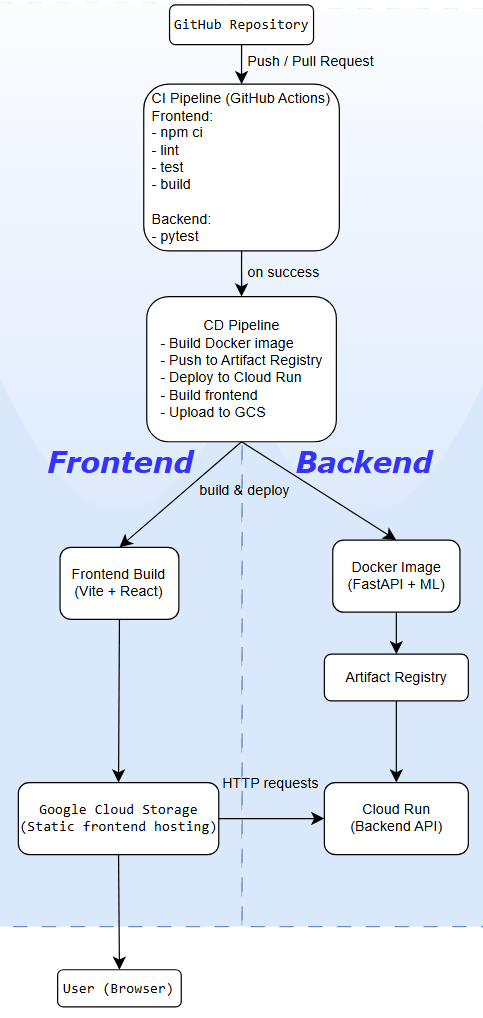
\includegraphics[width=0.5\textwidth]{figures/images/chapter-5/deployment-architecture.png}
\caption{Deployment architecture and CI/CD pipeline.}
\label{fig:deployment_architecture}
\end{figure}

Figure~\ref{fig:deployment_architecture} illustrates the deployment architecture
at a structural level. The frontend provides the user-facing interface and
communicates with the backend through HTTP-based API requests. By separating
presentation and interaction concerns from processing and inference, the system
becomes easier to maintain, update, and extend over time.

The deployment design also reflects the architectural principles presented
earlier in this chapter. In particular, the backend is treated as an isolated
service environment for processing and inference, while the frontend remains
focused on interaction and presentation. This supports modularity and reduces
coupling between the user interface and the underlying processing pipeline.
More specific technologies and infrastructure choices used to realize this
deployment are described in Chapter~\ref{chap:technologies_and_methodologies}.